% last updated in April 2002 by Antje Endemann
% Based on CVPR 07 and LNCS, with modifications by DAF, AZ and elle, 2008 and AA, 2010, and CC, 2011; TT, 2014; AAS, 2016

\documentclass[runningheads]{llncs}
\usepackage{graphicx}
\usepackage{amsmath,amssymb} % define this before the line numbering.
\usepackage{ruler}
\usepackage{color}
\usepackage{wrapfig}
\usepackage{makecell}
\usepackage{rotating}
\usepackage{enumitem}
\usepackage{multirow}
\usepackage{booktabs,tabu}
\usepackage[width=122mm,left=12mm,paperwidth=146mm,height=193mm,top=12mm,paperheight=217mm]{geometry}

\usepackage{cite} % automatically re-orders citation numbers

\usepackage{floatrow}

\newcommand\todo[1]{\textcolor{red}{#1}}

\newcommand\degr[0]{^{\circ}}


\begin{document}
% \renewcommand\thelinenumber{\color[rgb]{0.2,0.5,0.8}\normalfont\sffamily\scriptsize\arabic{linenumber}\color[rgb]{0,0,0}}
% \renewcommand\makeLineNumber {\hss\thelinenumber\ \hspace{6mm} \rlap{\hskip\textwidth\ \hspace{6.5mm}\thelinenumber}}
% \linenumbers
\pagestyle{headings}
\mainmatter

\def\ECCV18SubNumber{1114}

\title{Deep Photometric Stereo on a Sunny Day}
% Important keywords to highlight somehow in the title: Outdoor, One-Day, Sunny, PS, Deep

\titlerunning{ECCV-18 submission ID \ECCV18SubNumber}
\authorrunning{ECCV-18 submission ID \ECCV18SubNumber}

\author{Anonymous ECCV submission}
\institute{Paper ID \ECCV18SubNumber}


\maketitle

%  Given multiple images with different illumination taken from a single viewpoint, it is possible to recover the normals of the surfaces present in the scene. 
% Its application to outdoor scenes has seen recent interest. Unfortunately, most successful outdoor PS techniques requires either months of data or specific events to happen like an alternance of cloud occluding the sun.
\begin{abstract}
Photometric Stereo in outdoor illumination remains a challenging, ill-posed problem. Indeed, it has been shown that the scene structure cannot be recovered unambiguously from the photometric cues alone when it is lit by the sun over the course of a single day. In this paper, we present a CNN-based technique for photometric stereo on a single sunny day. We solve the ambiguity issue by combining photometric cues with prior knowledge on material properties, local surface geometry and the natural variations in outdoor lighting. To train the CNN, we create a dataset of realistic synthetic renders with both diffuse and specular materials. Given eight outdoor images taken during a single sunny day, our method robustly estimates the scene surface normals. Our approach does not require precise geolocation to work and significantly outperforms several state-of-the-art methods on images with real lighting. This shows that our CNN can combine efficiently learned priors and photometric cues available during a single sunny day.

\keywords{photometric stereo, deep learning, outdoor lighting}
\end{abstract}

% Even though the technique is robust to glossy materials, it requires a scene with uniform albedo and a camera pointing toward the North. 


%!TEX root = main.tex
\section{Introduction}

The biggest challenge in outdoor Photometric Stereo (PS) remains the fact that the sun, our main light source, moves along a trajectory that nearly lies on a plane throughout the course of the day, leaving the photometric reconstruction under-constrained~\cite{woodham-opteng-80}.
%Researchers have investigated different approaches to address this problem, which include collecting data for several months~\cite{abrams-eccv-12,ackermann-cvpr-12}, waiting for the best time of the year (around summer solstice in the North Hemisphere~\cite{shen-pg-14}) or, more recently, for a day with favorable atmospheric conditions (partly cloudy sky~\cite{holdgeoffroy-iccp-15,holdgeoffroy-3dv-15}).
As previously discussed, one way to circumvent this issue is to wait for partially cloudy days for the effective lighting direction to shift away from the solar plane.
In general, the practitioner has no control over the sun or the atmosphere and is therefore left with two options: ($i$) a potentially long wait for the ideal conditions to arise; or ($ii$) the use of a smarter reconstruction technique that does not rely solely on the photometric cue.

In this chapter, we investigate the second option above. By using machine learning to aggregate prior knowledge on the geometry and reflectance of common classes of objects, we aim to resolve the ambiguities cause by the limited photometric cues available in single-day outdoor PS. To avoid restricting the algorithm to a small family of objects, we build knowledge on local geometry based on the fact that complex surfaces are made up of simpler, piecewise smooth patches. Our approach is further motivated by the fact that material properties are also locally correlated within small surface patches. Working with a broad class of small surface patches keeps the approach general and also facilitates the collection of data for machine learning.

% While non-convolutional deep learning was already used in fully-constrained, indoor PS (mostly to learn a generic, ``inverse BRDF'' function)... 

As we reason in terms of surface patches, a natural choice is to follow a deep learning approach with a novel convolutional neural network (CNN) architecture to automatically learn features from image patches and guide 3D normal estimation. To our knowledge, this is the first CNN to address the problem of under-constrained, single-day outdoor PS.

Our CNN design seeks a balance between fully-calibrated PS (too restrictive) and uncalibrated PS (which introduces further ambiguities). We follow a semi-calibrated outdoor PS approach and only assume that: (1) the object is imaged at roughly predefined times of the day; (2) the sun is unobstructed by clouds at these times; and (3) an orthographic camera facing approximately north (or south). The latter assumption could be relaxed using recent advances on sun position estimation in the wild to automatically detect the camera orientation. One could then train our model on multiple camera calibrations and select the right one according to the detected orientation. Of note, our approach does not require known sun intensities nor complete geolocation data, as in previous work on outdoor PS~\cite{jung-cvpr-15}. Together, our assumptions define an ``8-figure'' subspace for the position of the sun through the year, known as an {\em analemma}, whose shape also varies with geographical location (fig.~\ref{fig:solar-analemma}).

% (PG: that's an assummed/given condition)
% camera (pointing north, orthographic projection)

% analemma (Wikipedia): position of the Sun in the sky over the course of a year, as viewed at a fixed time of day and from a fixed location on the Earth

Therefore, our outdoor PS network is required to learn priors not only on object materials and local geometry (diffuse, specular, smooth, ...), but also priors on lighting (variability in sun intensity and elevation with respect to geolocation and time of year). This knowledge is encoded in the network, which learns to output 3D normals as a non-linear function of input image patches taken throughout a day. This rich prior knowledge allows us to obtain a reconstruction performance that outperforms the current state-of-the-art on real lighting data with only 3 images, which is much lower than the 6-18 typically used by previous work~\cite{yu-iccp-13,jung-cvpr-15}. Our fully trained method will be made publicly available.

%To train our CNN, we realistically render synthetic datasets with a large variety of image patches with different geometry, materials and lighting.

%\todo{Say something about the quality of our results vs state of the art.}

We summarize our contributions as follows:
\begin{itemize}[noitemsep,nolistsep]
	\item a state-of-the-art method for single-day photometric stereo on sunny days that is robust to shadows, specularities and arbitrary but uniform albedo;
    \item a pipeline to generate synthetic images with a mix of Lambertian and glossy materials that captures the diversity of real outdoor lighting.
\end{itemize}


%!TEX root = main.tex
\chapter{Related Work}

In this chapter, we will cover the literature of the two main axes of research presented. First, an overview of the recent literature on photometric stereo is presented. An emphasis is put on dealing with various illumination conditions, from controlled laboratory conditions to the harder outdoor lighting case. Then, a review of prior art in lighting and camera calibration is discussed. For the latter, we will mainly focus on horizon line estimation, which provides the main extrinsic parameters with respect to the earth.


\section{Photometric Stereo}


As shown in Woodham's seminal work~\cite{woodham-opteng-80}, for Lambertian surfaces, calibrated PS computes a (scaled) normal vector in closed form as a simple linear function of the input image pixels; this linear mapping is only well-defined for images obtained under three or more (known) non-coplanar lighting directions.
% intro on PS
Since its inception in the early 80s, it has been explored under many an angle. Whether it has been to improve its ability to deal with complex materials~\cite{alldrin-cvpr-08}, lighting conditions~\cite{alldrin-cvpr-08,basri-ijcv-07,johnson-cvpr-11,oxholm-eccv-12} or enhance other techniques like multiview stereo~\cite{snavely-ijcv-08}, the myriad of papers published on the topic are testament to the interest this technique has garnered in the community. A more detailed overview of general PS can be found in the recent, excellent review in~\cite{shi-tpami-18}. While most of the papers on this topic have focused on images captured in the lab, recent progress has allowed the application of PS on images captured outdoors, lit by the more challenging case of uncontrollable, natural illumination. 

% ask the question: how many images do we need?
A central question to any PS practitioner is that of the quality and amount of data required to achieve good performance. What should the lighting conditions be during data capture? How many images (illumination conditions) are needed? What is the shortest time interval required to collect these samples?

In the lab, theoretical analyses for Lambertian surfaces, lit by point light sources, reveal that the minimum number of images is three~\cite{woodham-opteng-80} and that the optimal light configuration yields an orthogonal triplet of light directions~\cite{drbohlav-iccv-05}. While such theoretical guarantees are reassuring, they are however much harder to obtain for the case of more complex, non-Lambertian reflectance, or with more general lighting models. Thus, practitioners are left without guidance in the task of determining when to stop capturing data, an inherently tedious trial-and-error process. As a result, it is not rare for PS datasets to include hundreds of images~\cite{alldrin-cvpr-08} in an uncertain attempt to obtain accurate reconstruction.

Subsequent work on outdoor PS has struggled to meet the light non-coplanarity requirement since, over the course of a day, the sun shines from directions that nearly lie on a plane. These co-planar sun directions then yield an ill-posed problem known as two-source PS; despite extensive research using integrability and smoothness constraints~\cite{onn-ijcv-90,hernandez-pami-11}, results still present strong regularization artifacts on surfaces that are not smooth everywhere. To avoid this problem in outdoor PS, authors initially proposed gathering months of data, watching the sun elevation change over the seasons~\cite{abrams-eccv-12,ackermann-cvpr-12}. More recently, Shen~{\em et al.}~\cite{shen-pg-14} noted that the coplanarity of the daily sun directions actually varies throughout the year, with single-day outdoor PS becoming more ill-posed at high latitudes near the winter solstice, and worldwide near the equinoxes. A creative solution to this problem was proposed in~\cite{hung-wacv-15}, but it is limited to objects that can be placed on a small moving platform. Therefore, capturing more data for fixed, large objects meant until recently waiting days, or even months, potentially~\cite{ackermann-cvpr-12,abrams-eccv-12}. 

% richer lighting models
To compensate for limited sun motion, other approaches use richer illumination models that account for additional atmospheric factors in the sky. This is done by employing \mbox{(hemi-)spherical} environment maps~\cite{debevec-siggraph-98} that are either real sky images~\cite{yu-iccp-13,shi-3dv-14,hung-wacv-15} or synthesized by parametric sky models~\cite{inose-tcva-13,jung-cvpr-15}. Using a large database of real sky images, Hold-Geoffroy~{et al.}~\cite{holdgeoffroy-iccp-15} showed that partly cloudy days are in fact better for single-day outdoor PS since clouds obscure and further scatter sun light, causing an out-of-plane shift in the effective direction of illumination. Subsequently~\cite{holdgeoffroy-3dv-15}, they also showed that good cloud coverage conditions for stable solutions may be observed in the sky within very short time intervals of just above one hour.

%While capturing more data in the lab can be done relatively easily, the same cannot be said for outdoor imagery. Indeed, one does not control the sun and the other atmospheric elements in the sky; so one must wait for lighting conditions to change on their own. 

%Luckily, techniques that reduce the requirement to a single day's worth of data have also been proposed~\cite{yu-iccp-13,shen-pg-14,jung-cvpr-15}. However, this is still much longer than what can be done in the lab, where light sources can be waved around rapidly and data be captured in minutes. And although recent work has investigated which days provide more favorable atmospheric conditions for outdoor PS~\cite{shen-pg-14}, so far, no study has systematically demonstrated the performance of outdoor PS with less than a full day's worth of data.


% solar plane, nearly singular (ill-conditioned) light matrix, 2-image PS
% regularization breaks at (sharp) surface discontinuities

% webcams, solar plane

Despite these developments, state-of-the-art approaches in calibrated~\cite{yu-iccp-13} and semi-calibrated~\cite{jung-cvpr-15} (based on precise geolocation) outdoor PS are still prone to potentially long waits for ideal conditions to arise in the sky; and verifying the occurrence of such events is still a trial-and-error process. So far, deep PS had only been applied in indoor scenarios with rich and controlled illumination~\cite{yu-iccv-17,santo-iccv-17,taniai-arxiv-18,shi-tpami-18}, focusing on learning inverse functions for non-Lambertian reflectances.

%\cite{yu-iccv-17,santo-iccv-17,taniai-arxiv-18} Deep learning methods applied to photometric stereo (not one-day)

% Talk about DiLiGent~\cite{shi-tpami-18}? (Their objects have homogeneous material, with piecewise constant albedo, our method would work with any albedo pattern using the division trick. Also, only normal maps, no 3D models. Their sampling of 96 lighting directions does not approximate well the path of the sun through a day.)

% single image (nishino, deep learning)
Finally, under more extreme ambiguity, techniques for shape-from-shading (SfS)~\cite{Horn1989,Zhang1999,Langer1994,oxholm-eccv-12,johnson-cvpr-11,barron-pami-15} attempt to recover 3D normals from a single input image, in which case the shading cue alone is obviously insufficient to uniquely define a solution. Thus, SfS relies strongly on priors of different complexities and deep learning is quickly bringing advances to the field~\cite{eigen-iccv-15,shu-cvpr-17,wu-nips-17,shu-cvpr-17}.



\section{Lighting calibration}

Lighting is the fundamental element that makes up all images. As Paul Cézanne said, ``there is no model; there is only color.'' Knowing the lighting of a scene allows for a deeper understanding of the camera, the scene and its materials.

In this section, we will focus on outdoor illumination models and algorithms to estimate them and related inverse rendering approaches.

\subsection{Analytical outdoor illumination models}

Analytical sky models are composed of a single empirically-derived closed-form equation to obtain the luminance of the sky. While they are typically used for rendering and real-time applications because of their high evaluation speed.

The first weather condition that was modeled is the overcast sky. Kimball and Hand~\cite{kimball1921sky} were the firsts to report in 1921 that cloudy days had higher luminosity near their zenith, and decreasing luminosity toward the horizon. Moon and Spencer~\cite{moon1942illumination} formulated the first luminance distribution model for the overcast sky in 1942. This work has been revisited and adopted as the CIE overcast sky model in 1996~\cite{cie1996s}. In this model, the luminance of the sky $Y_z$ in function of the zenith angle $\theta$ is defined as
\begin{equation}
Y_z = \frac{1 + 2 \; \cos\left( \theta \right)}{3} \quad.
\end{equation}
To summarize, the sky luminance of overcast days is proportional to the $\cos$ of the zenith angle. While this model predicts quite accurately overcast days, it does not tell the whole story about daylight in general.

For more general, non-overcast skies, Kittler~\cite{kittler1985luminance} was the first to propose a luminance distribution measurement strategy and predictive model, which eventually became the CIE standard sky model~\cite{darula-cie-sky}. Based on this model, Perez et al.~\cite{perez1993allweather} proposed a generalization called the all-weather sky luminance distribution model. This model is parameterized by five coefficients that can be varied to generate a wide range of skies. Preetham~\cite{preetham-siggraph-99} proposed a simplified version of the Perez model that derives the five coefficients from a single unified atmospheric turbidity parameter, which they fit on physical simulations. Eight years later, a critic of this Preetham model is published~\cite{zotti2007critical}, relating the relatively small valid turbidity range, the systematically too bright antisolar region and the too smooth intensity peak toward the sun. Most of those issues were solved by Ho\v{s}ek and Wilkie, which proposed a sky luminance model~\cite{hosek-siggraph-12}, still parameterized by this same turbidity parameter. In subsequent work, they extended it to include a solar radiance function~\cite{hosek-cga-13} and earth-like extrasolar skies~\cite{wilkie2013predicting}. Lalonde and Matthews~\cite{lalonde-3dv-14} also contributed to solving those issues by combining the Preetham sky model with a novel empirical sun model.

\subsection{Physically-based outdoor illumination models}

Contrarily to analytical models, physically-based models are based on physical simulations to provide a luminance distribution. They are usually slower but typically closer to real sky luminance measurements than analytical models.

The first model to explain the principal physical phenomenons coming into play to form daylight was published by Nishita et al. in their seminal work of 1993~\cite{nishita1993display}. They explain that two types of interactions with the electromagnetic field dominate the sky appearance. The first one concerns clear skies, modeling interactions with small aerosols. Specifically, it encompasses particles with a radius $r$ significantly smaller than the light wavelength $\lambda$ ($\frac{2\pi r}{\lambda} \ll 1$). This case of interactions is called the Rayleigh scattering and predicts the interactions with nitrogen and hydrogen, the major constituents of air. This is the reason why the sky is perceived blue. The second type of interactions solves Maxwell's equations for the case of particles with a radius $r$ roughly the same size as the light wavelength $\lambda$ ($\frac{2\pi r}{\lambda} \approx 1$). It represents interactions of light with heavier molecules like water particles in suspension in the atmosphere, in clouds or during fog. This class of interactions is called the Mie scattering. Summing both Rayleigh and Mie scattering together gives luminance estimations very close to the measurements performed during daylight, confirming the dominance of those two phenomenons for the appearance of the sky.

This sum of both Rayleigh and Mie scattering is also used as reference when developing the Preetham~\cite{preetham-siggraph-99} and Ho\v{s}ek-Wilkie~\cite{hosek-siggraph-12} analytical models. The parameters of those analytic models were fit to the physical simulations of both Rayleigh and Mie scattering using either a least square quadratic optimization or a spline, respectively.

In subsequent work, Nishita et al.~\cite{nishita1996display} enhanced their model by adding two elements: 1) the influence of ground albedo on the sky and 2) multiple scattering, meaning considering more than a single interaction before observation like their previous publication.

Most published physically-based models are variants of the Rayleigh and Mie scattering proposed in~\cite{nishita1993display}, usually focusing on speeding up the simulation~\cite{oneal2005accurate}, increasing agreement with measures~\cite{haber2005physically,bruneton2008precomputed} or extending it to arbitrary atmospheres like oceans~\cite{elek2010real}.

Daylight is not the only phenomenon that received attention in the literature. A night sky model has also been developed~\cite{jensen2001nightskymodel}, taking into consideration the sun's reflection on the moon as well as the light emitted from the stars.

\subsection{Outdoor lighting estimation}

Lalonde et al.~\cite{lalonde-ijcv-12} combine multiple cues, including shadows, shading of vertical surfaces, and sky appearance to predict the direction and visibility of the sun. This is combined with an estimation of sky illumination (represented by the Perez model~\cite{perez1993allweather}) from sky pixels~\cite{lalonde-ijcv-10}. Similar to this work, we use a physically-based model for outdoor illumination. However, instead of designing hand-crafted features to estimate illumination, we train a CNN to directly learn the highly complex mapping between image pixels and illumination parameters. 

Other techniques for single image illumination estimation rely on known geometry and/or strong priors on scene reflectance, geometry and illumination~\cite{barron-pami-15,barron2013rgbd,lombardi2016reflectance}. These priors typically do not generalize to large-scale outdoor scenes. Karsch et al.~\cite{karsch2014automatic} retrieve panoramas (from the SUN360 panorama dataset~\cite{xiao-cvpr-12}) with features similar to the input image, and refine the retrieved panoramas to compute the illumination. However, the matching metric is based on image content which may not be directly linked with illumination. 

Another class of techniques simplify the problem by estimating illumination from image collections. Multi-view image collections have been used to reconstruct geometry, which is used to recover outdoor illumination~\cite{haber2009relighting,lalonde-3dv-14,shan2015visual,duchene2015multiview}, sun direction~\cite{wehrwein2015shadows}, or place and time of capture~\cite{hauagge2014outdoor}. Appearance changes have also been used to recover colorimetric variations of outdoor sun-sky illumination~\cite{sunkavalli2008color}. 

\subsection{Inverse graphics/vision problems in deep learning}

Following the remarkable success of deep learning-based methods on high-level recognition problems, these approaches are now being increasingly used to solve inverse graphics problems~\cite{kulkarni15dcign}. In the context of understanding scene appearance, previous work has leveraged deep learning to estimate depth and surface normals~\cite{eigen-iccv-15,bansal2016marr}, recognize materials~\cite{bell2015minc}, decompose intrinsic images~\cite{zhou2015intrinsic}, recover reflectance maps~\cite{rematas-cvpr-16}, and estimate, in a setup similar to physics-based techniques~\cite{lombardi2016reflectance}, lighting from objects of specular materials~\cite{georgoulis2016delight}. We believe ours is the first attempt at using deep learning for full HDR outdoor lighting estimation from a single image.


\section{Camera calibration}

Geometric camera calibration is a widely studied topic that has a significant impact on a variety of applications including metrology~\cite{Criminisi2000}, 3D inference~\cite{Criminisi00,Fouhey2013} and augmented reality, both indoor~\cite{hedau-iccv-09,izadinia-cvpr-17} and outdoor~\cite{hoiem-cvpr-06}. As such, many techniques were developed to perform precise geometric calibration using a calibration target inserted beforehand in the image~\cite{Sturm1999,Zhang2002,Heikkila1997,Chen2004}. For after-the-fact calibration, most work on camera calibration aim to detect specific geometric objects in the image typically present in human-made environments~\cite{Rother2000,Melo2013}. Similarly, PoseNet~\cite{kendall-iccv-15} performs camera relocalization by jointly learning location and orientation. More recently, methods for straighting up photographs like Upright~\cite{Lee2014} recover calibration by finding vanishing points. Other work proposed to take advantage of lighting cues to calibrate~\cite{lalonde-ijcv-10,Workman2014}, circumventing the need for human-made environments. However, these techniques often fail on complex scenes where semantic reasoning is required to discard misleading textures and visual cues. To solve the need for high-level reasoning, deep convolutional neural networks were recently used to estimate field of view~\cite{Workman2015a} and horizon lines~\cite{Workman2016}, bringing camera calibration on single images to a wider variety of scenes.

Understanding the limits of the human visual system has also received significant attention, with studies quantifying color sensitivity~\cite{fairchild2013color}, how reliably we can detect photo manipulations artifacts~\cite{Farid2010} and how people perceive distortion in street-level image-based rendering~\cite{Vangorp2013}. More recently, perceptual studies were performed to assess human appreciation on tasks like super-resolution~\cite{ledig-cvpr-17}, image caption generation~\cite{vinyals-cvpr-15} and video temporal alignment~\cite{papazoglou-accv-16}.


% %!TEX root = main.tex
\section{Image calibration network}
\label{sec:ch4_proposed_method}

In this section, we present our CNN architecture for single image calibration  and compare it to the state-of-the-art estimation method.  To train this model, we need a large number of images and their corresponding camera parameters. However, no such dataset currently exist. Structure from Motion (SfM) datasets~\cite{Wilson2014} provides relatively accurate field of view values but no horizon lines, and conversely the Horizon Lines in the Wild (HLW) dataset~\cite{Workman2016} provides horizon lines but no field of view. In the following, we discuss how we generate our camera calibration dataset, how the CNN model was trained, and we use guided backpropagation to analyze the image features the model focuses on to provide its estimations, which gives insights into the cues that are important to perform camera calibration. 

\subsection{Dataset}
\label{sec:dataset_generation}

\begin{table}[!t]
\centering
\footnotesize
\begin{tabular}{lll}
\toprule
Parameter & Distribution & Values \\
\midrule
Focal length (mm) & Lognormal & $\mu=14, \sigma=17$ \\
Horizon (pixels) & Normal & $\mu=0.046, \sigma=0.3$ \\
Roll ($^\circ$) & Cauchy & $x_0 = 0$, $\gamma \in \{0.001, 0.1\}$ \\
Aspect ratio & Varying & $\{1{:}1, 5{:}4, 4{:}3, 3{:}2, 16{:}9\}$ \\
\bottomrule
\end{tabular}
\vspace{1em}
\caption{Sampling of camera parameters used to generate the dataset for the human sensitivity study.}
\label{tab:parameters-sampling}
\end{table}

Our goal is to train a deep network to estimate the camera roll, pitch, and field of view from a single image. To obtain images and their ground truth camera parameters, we take inspiration from \cite{Workman2016,holdgeoffroy-cvpr-17} and leverage the SUN360 database~\cite{Xiao2012}, which contains a large number of $360^\circ$ panoramas. We extract 7 rectified images from each panorama using a standard pinhole camera model of random parameters. To obtain reasonable camera parameters, the sampling strategies indicated in table~\ref{tab:parameters-sampling} were employed. Note that for the camera roll, two different Cauchy distributions are sampled with 0.33 and 0.66 probability respectively. This was done to model the fact that many photos typically have a roll close to 0. The aspect ratios were chosen by sampling Flickr and ImageNet images. Note that a larger probability (0.66) was given to the $4{:}3$ aspect ratio as it is the most common. The other aspect ratios are given a probability of $0.11$. We resize the extracted images to $224\times224$ to fit the neural network input size. This results in a dataset of 399,728 pairs of photos and their corresponding camera calibration which we split into a training set of 389,760 pairs, a validation set of 9,078 pairs and a test set of 890 pairs. Special care was taken to ensure no panorama used in the training set was present in validation or test set through other cropped photos.

As in~\cite{Workman2016}, we use the slope/offset ($\psi,\rho$) representation, where the horizon line is parameterized by the roll $\psi$ and its perpendicular distance from the center of the image $\rho$.

\subsection{Architecture}

We adopt a DenseNet~\cite{Huang2016} model pretrained on ImageNet~\cite{Russakovsky2015} on which we replace the last layer with three separate heads: one for estimating the horizon angle $\psi$, a second one to estimate the horizon's distance to the center of the image $\rho$ and a third one to estimate the vertical field of view of the image $h_{\theta}$.
All output layers use the softmax activation function to output a probability distribution by discretizing their respective parameter into 256 bins. This type of representation was also used in~\cite{Workman2016}. Fitting a standard distribution to the CNN output bins gives a sense of the uncertainty of the estimation, which is not possible to obtain when performing a regression as the CNN output is a single value. We adopt a range of $\left[ -\nicefrac{\pi}{2}, \nicefrac{\pi}{2} \right]$ for slope and $\left[ -1.6, 1.6\right]$ for offset. For both parameters, we use smaller bins around 0 for finer estimations around those values. Bin width follow an inverse normal distribution with $\mu=0,\, \sigma=\left\{ 0.5, 1 \right\}$ for slope and offset, respectively. We sum the Kullback-Leibler divergence of the three heads and use it as loss to train the model, which we minimize using stochastic gradient descent with the Adam optimizer~\cite{kingma-iclr-15} with an initial learning rate of $\eta = 0.001$ and a learning rate decay of $ \alpha = 0.0002$. Training is performed on mini-batches of 42 images. Convergence is observed through early stopping typically after 9-10 epochs, presumably because of the large size of our training set and our use of transfer learning through a pretrained model.

\begin{figure}
\centering
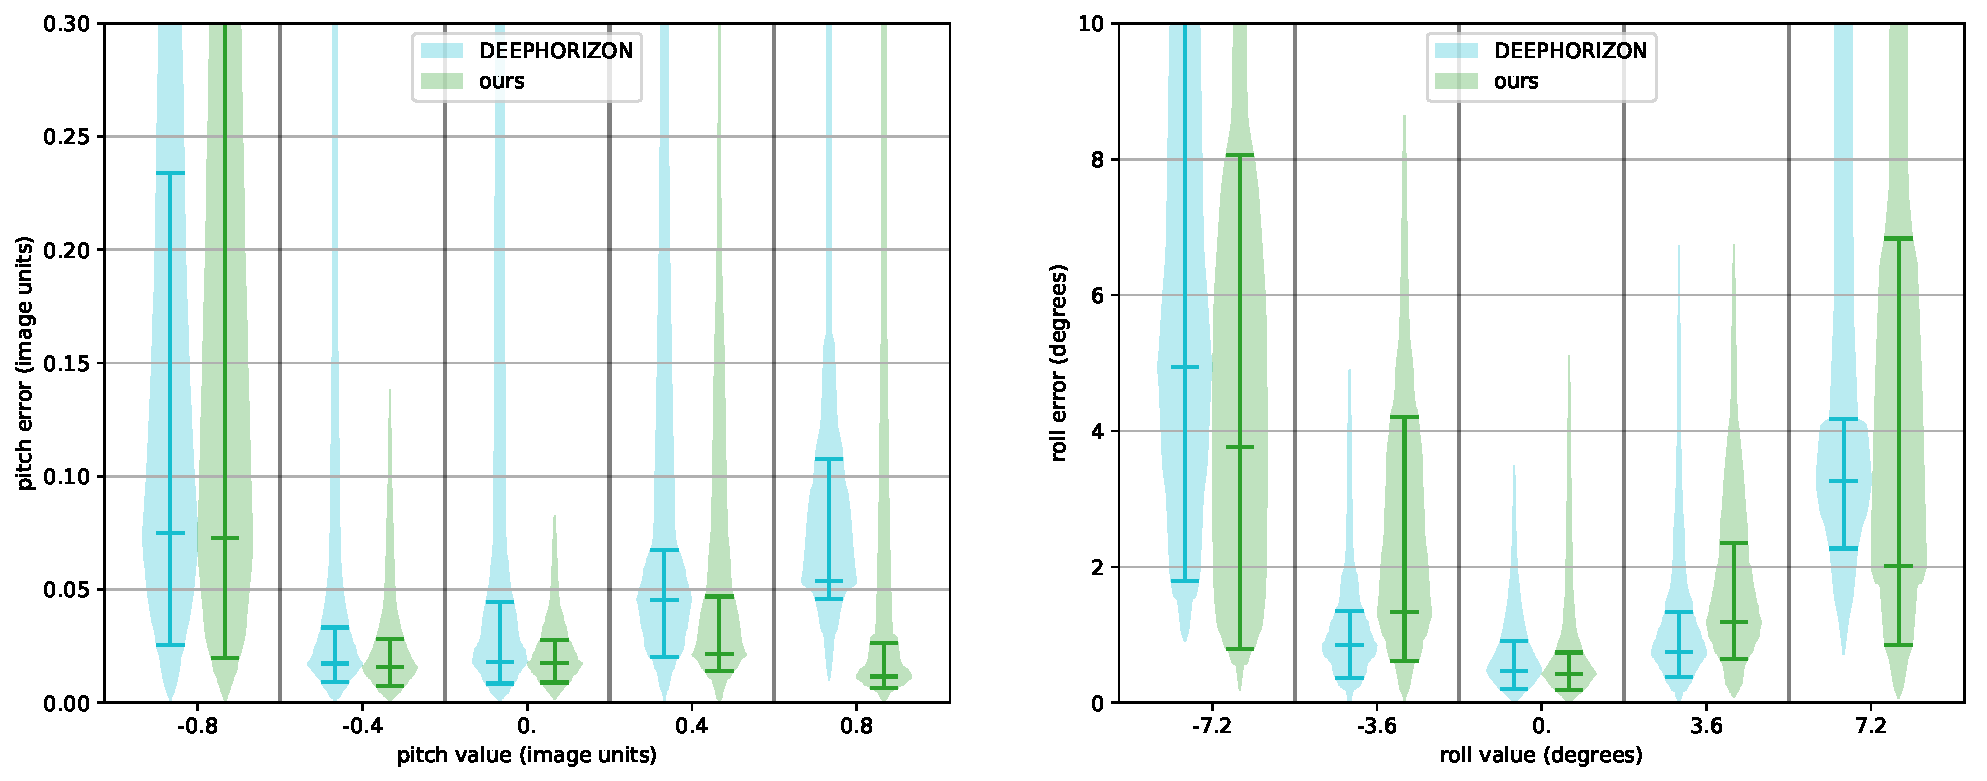
\includegraphics[width=\linewidth]{figures/method/pitch_roll_performance_hlw.pdf} \\
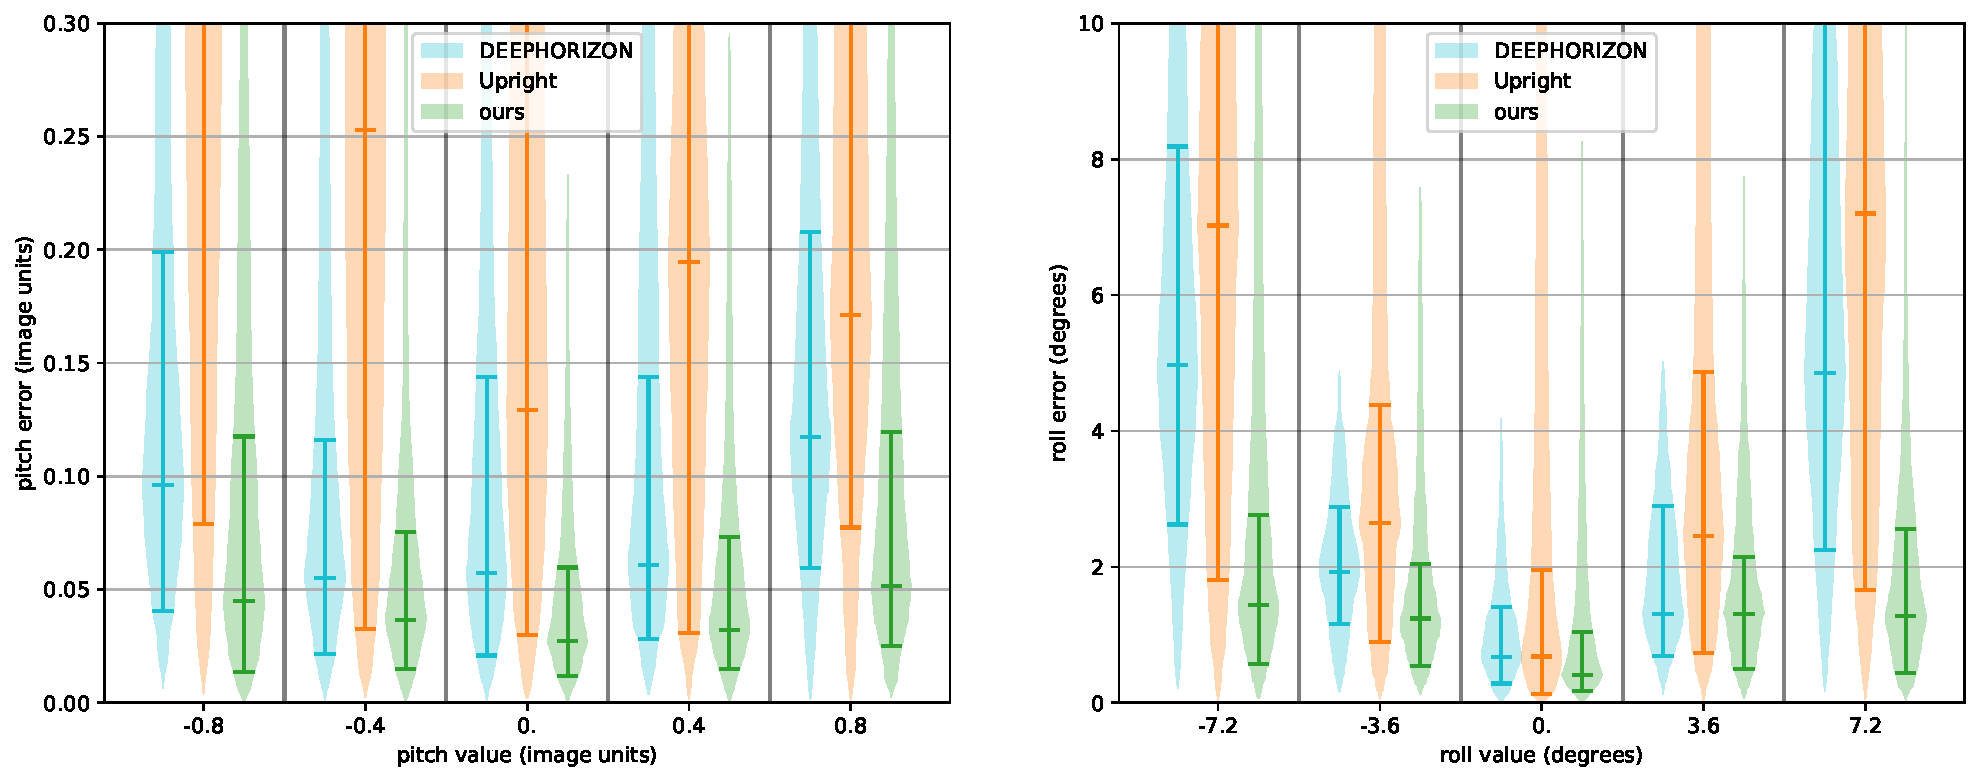
\includegraphics[width=\linewidth]{figures/method/pitch_roll_performance_sun360.pdf}
\caption[Pitch and roll estimation performance]{Pitch (left) and roll (right) estimation performance on the HLW dataset (top) and our SUN360 test set (bottom). Negative pitch denotes a camera pointing up. Results are displayed as "box-percentile plots"~\cite{esty-jss-03}, where the envelope of each column represents the percentile and the horizontal bars represents the first quartile, median and third quartile. Estimation errors (y-axis) are grouped into bins according to the parameter value (x-axis).}
\label{fig:method_pitch_roll_performance}
\end{figure}

\begin{figure}
\centering
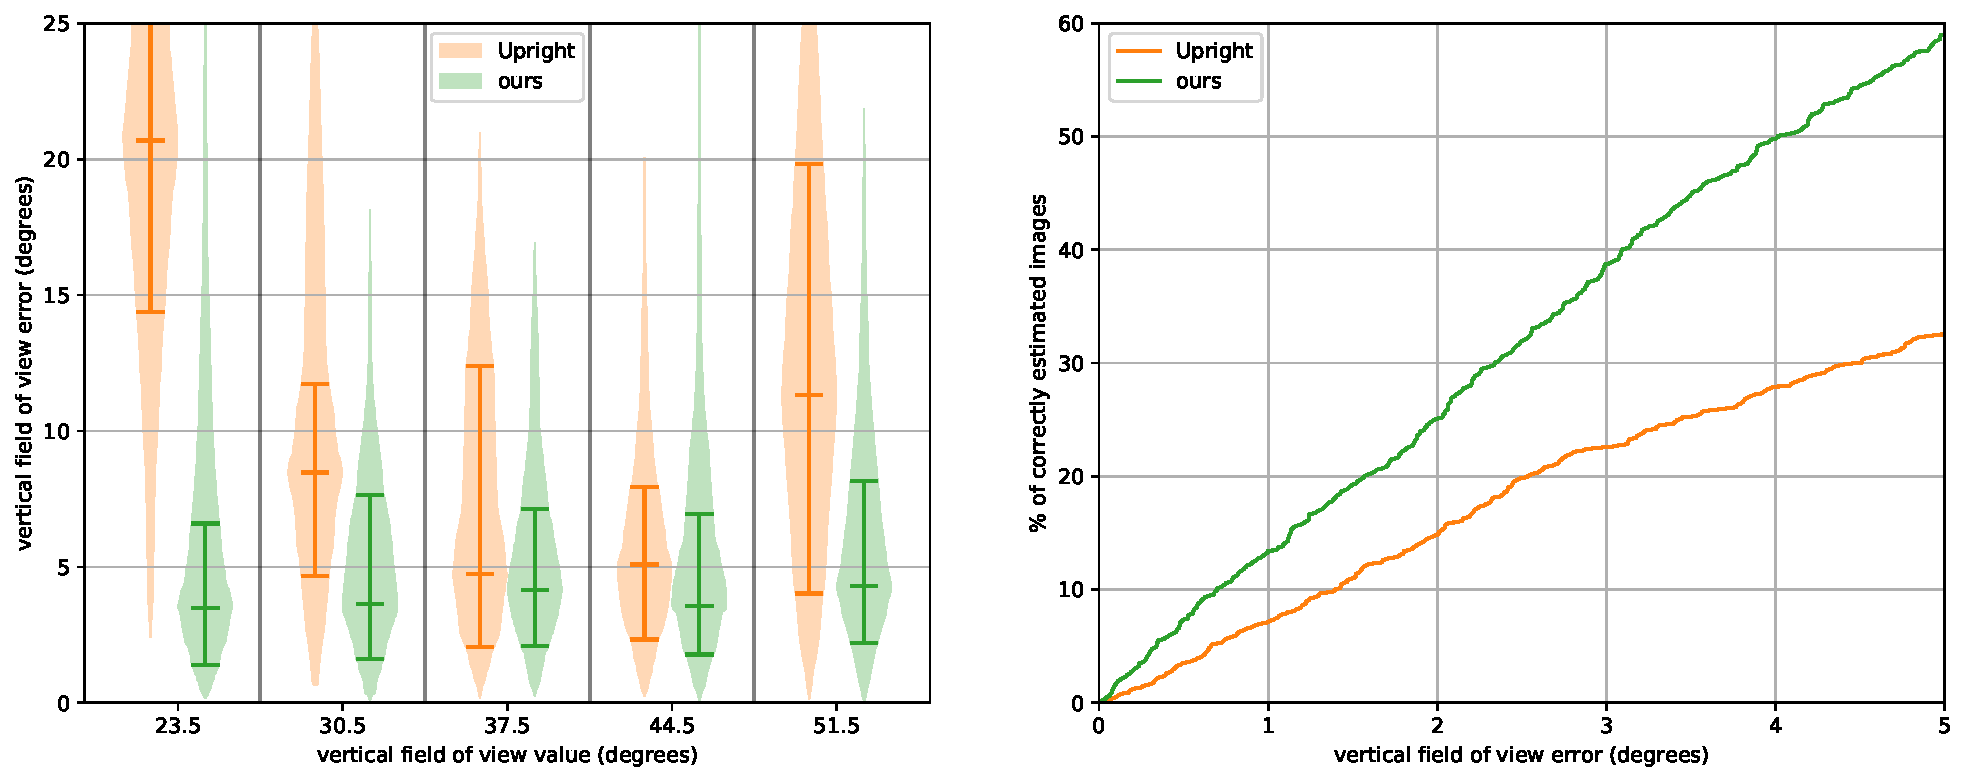
\includegraphics[width=\linewidth]{figures/method/vfov_performance_sun360.pdf}
% \includegraphics[width=\linewidth]{figures/method/vfov_performance_1dsfm.pdf}
\caption[Field of view estimation performance]{Vertical field of view estimation performance on our SUN360 test set displayed as a "box-percentile plot" (left) and a cumulative distribution function (right). See fig.~\ref{fig:method_pitch_roll_performance} for an explanation of the box-percentile plot.
%For the 1DSFM dataset, we also show the performance one would obtain by estimating systematically 38.4\degree, the dataset's median. See fig.~\ref{fig:method_vfov_onedsfm_diversity} for an overview of the diversity of both datasets.
}
\label{fig:method_vfov_performance}
\vspace{-1em}
\end{figure}

% \begin{figure}
% \centering
% \includegraphics[width=\linewidth]{figures/method/vfov_1dsfm_diversity.pdf}
% \caption{Diversity of field of views in our SUN360 test set (left) and the 1DSFM test set (right).}
% \label{fig:method_vfov_onedsfm_diversity}
% \vspace{-1em}
% \end{figure}

\section{Evaluation}

We report quantitative horizon line estimation performance of Upright~\cite{Lee2014}, DEEPHORIZON~\cite{Workman2016} (as trained by the authors) and our method (trained on SUN360) on two different datasets, the Horizon Lines in the Wild (HLW) dataset~\cite{Workman2016} and our SUN360 test set in fig.~\ref{fig:method_pitch_roll_performance}. We observe that aside from large roll errors on HLW, our method outperforms the state-of-the-art in most cases. Upright fails to converge on many cases since multiple images in our SUN360 test set do not contain edges on which the technique relies on. Qualitative results are shown in fig.~\ref{fig:method_example_results}.

Fig.~\ref{fig:method_vfov_performance} shows the quantitative field of view estimation performance on our SUN360 test set.
% and DEEPFOCAL's subset of the 1DSFM dataset~\cite{Workman2015a} 
Our method significantly outperforms Upright~\cite{Lee2014} across the entire range of parameters.
% For the 1DSFM dataset, we also provide the performance when the estimation is always the median of this dataset, 38.4\degree, which puts almost 60\% of the estimations within 5\degree error. We show the diversity of fields of view in both our SUN360 test set and 1DSFM (fig.~\ref{fig:method_vfov_onedsfm_diversity}). Note that no ground truth field of view is available for the HLW dataset and no horizon line annotations are provided with the 1DSFM dataset.



\newcommand{\sgbpwidth}{0.2}
\begin{figure*}
\centering
\bgroup
\def\arraystretch{0}
\begin{tabular}{@{}c@{}c@{}c@{}c@{}c@{}}
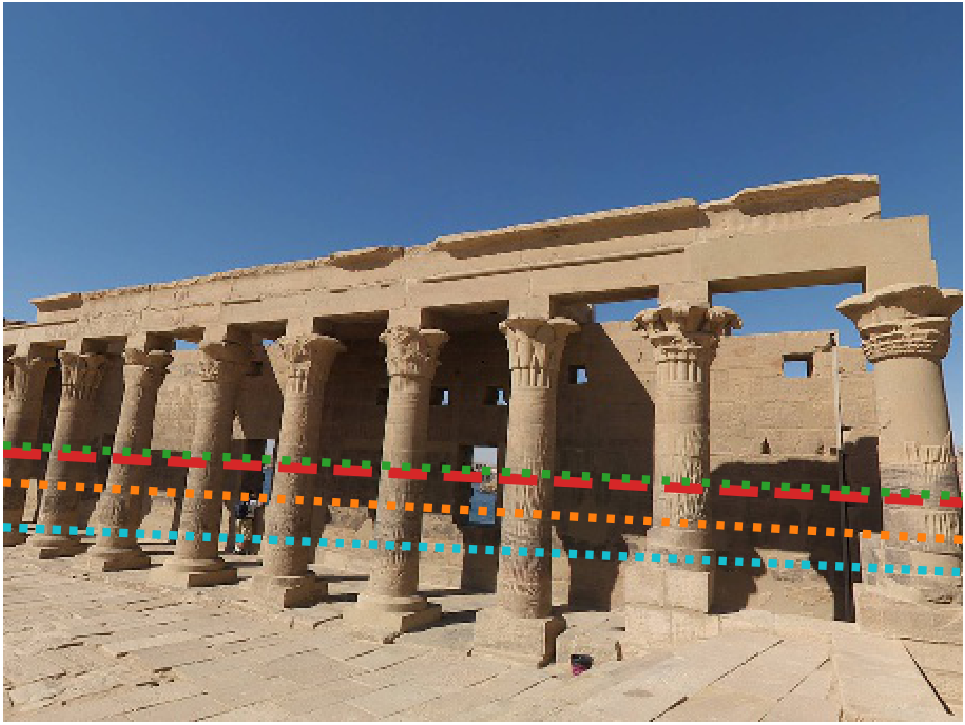
\includegraphics[width=\sgbpwidth\linewidth]{figures/nn_analysis/sgbp/pano_addbhhhqoevobx_jpg-1.png} &
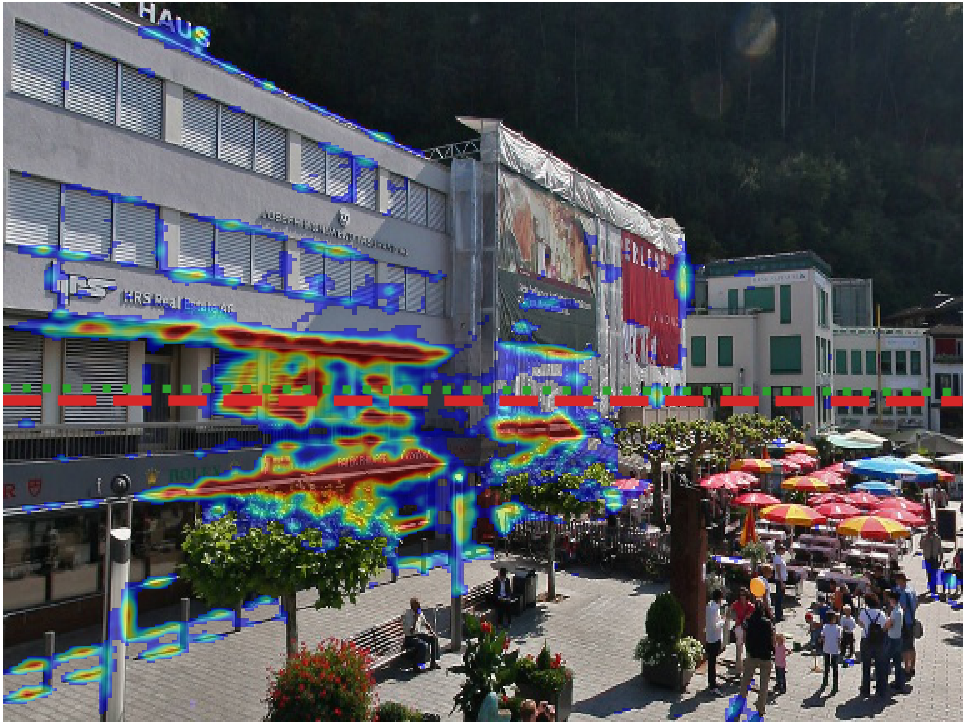
\includegraphics[width=\sgbpwidth\linewidth]{figures/nn_analysis/sgbp/pano_addfjqyibbzulh_jpg-2.png} &
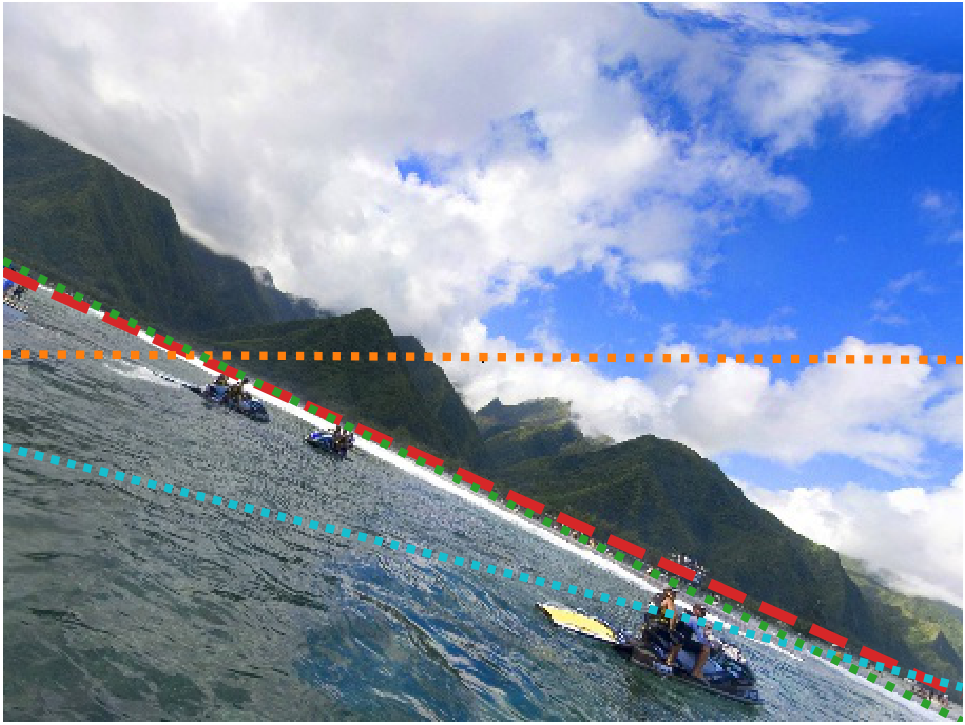
\includegraphics[width=\sgbpwidth\linewidth]{figures/nn_analysis/sgbp/pano_addgasjevqjafh_jpg-1.png} &
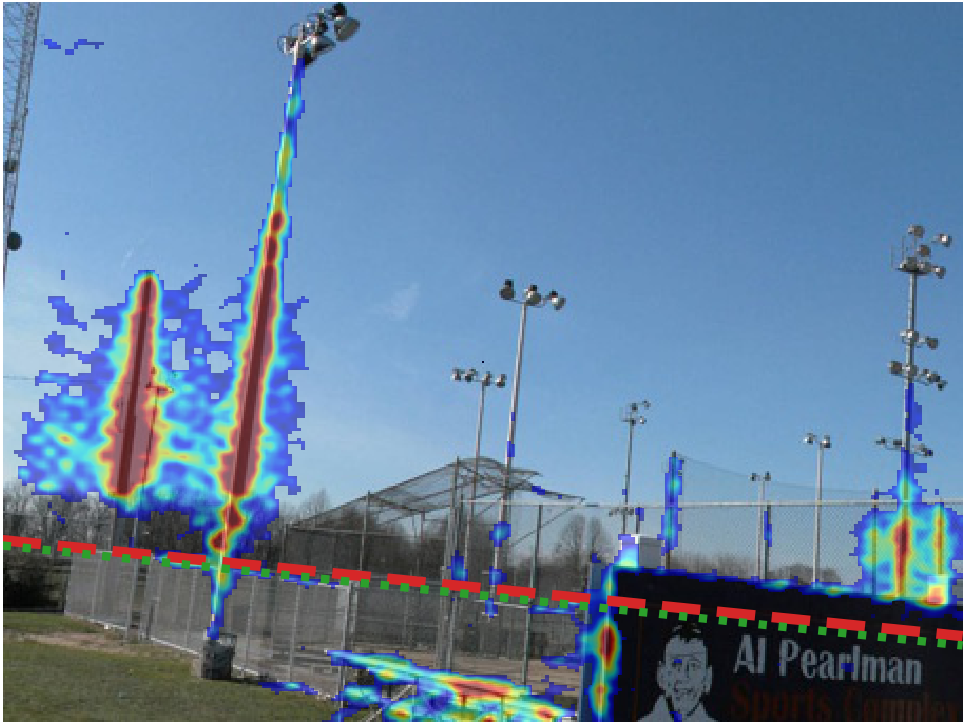
\includegraphics[width=\sgbpwidth\linewidth]{figures/nn_analysis/sgbp/pano_ayfwzaseviqbww_jpg-2.png} &
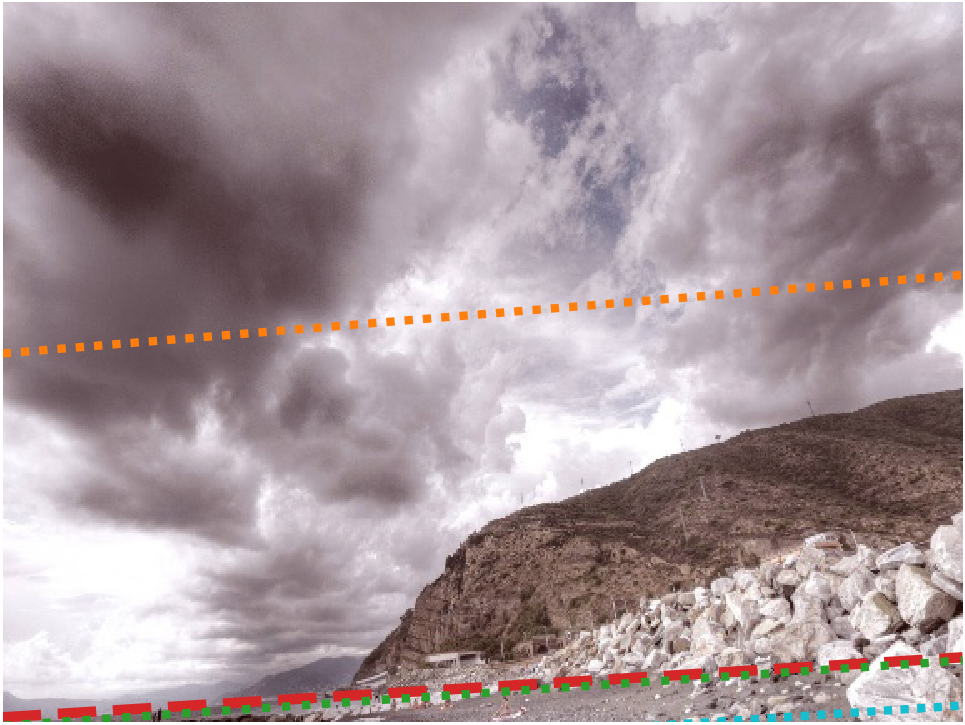
\includegraphics[width=\sgbpwidth\linewidth]{figures/nn_analysis/sgbp/pano_addtfngrqwwyvb_jpg-6.png} \\
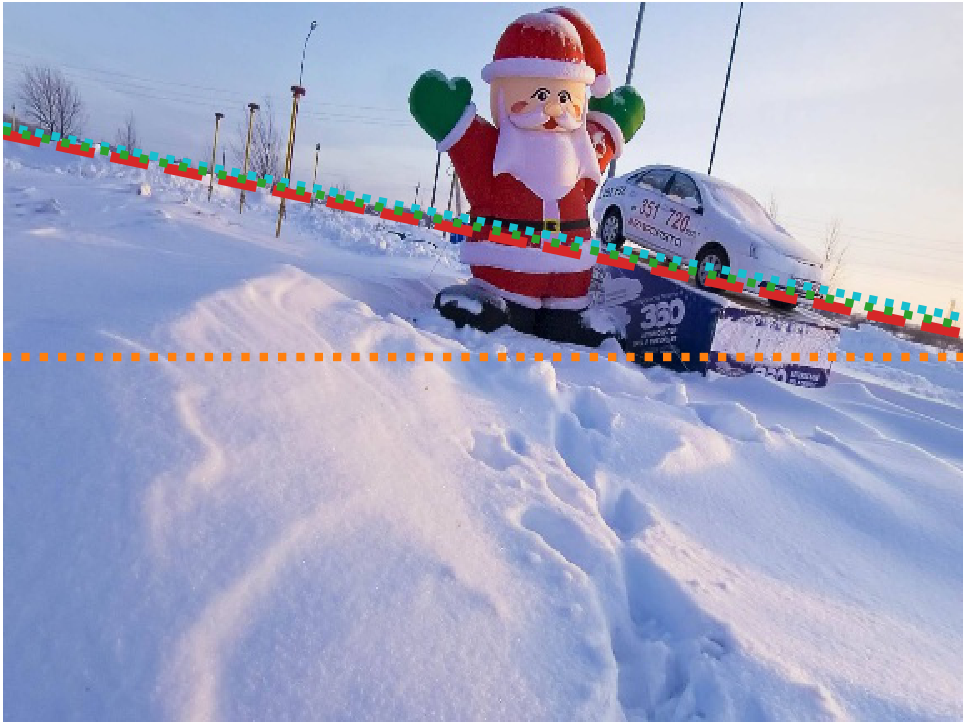
\includegraphics[width=\sgbpwidth\linewidth]{figures/nn_analysis/sgbp/pano_addtwdtklktubg_jpg-3.png} &
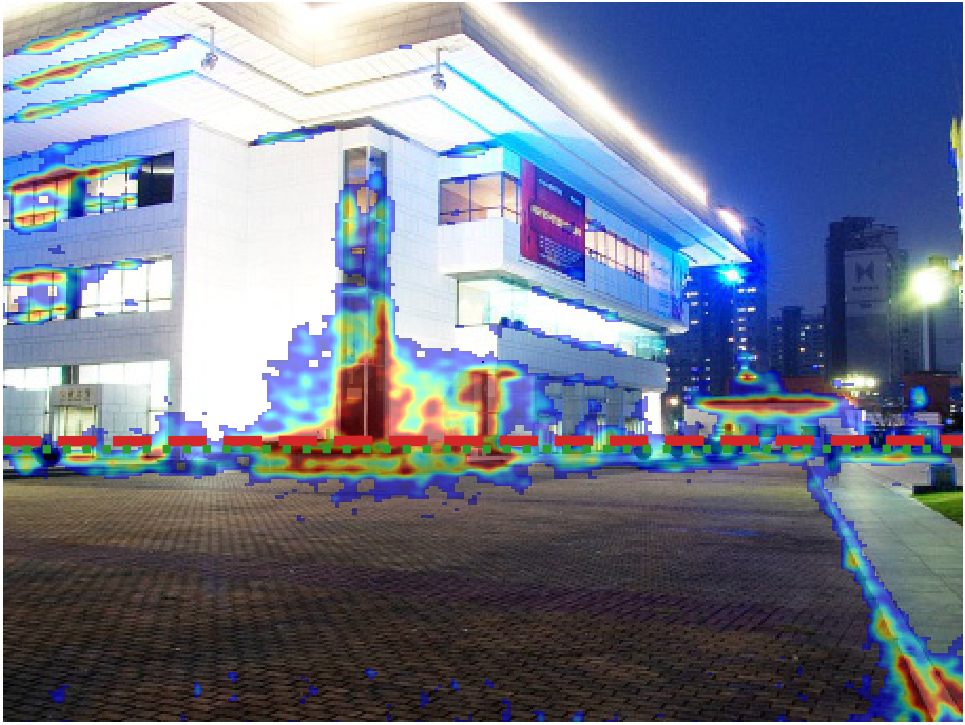
\includegraphics[width=\sgbpwidth\linewidth]{figures/nn_analysis/sgbp/pano_ayflzrhzcccird_jpg-4.png} &
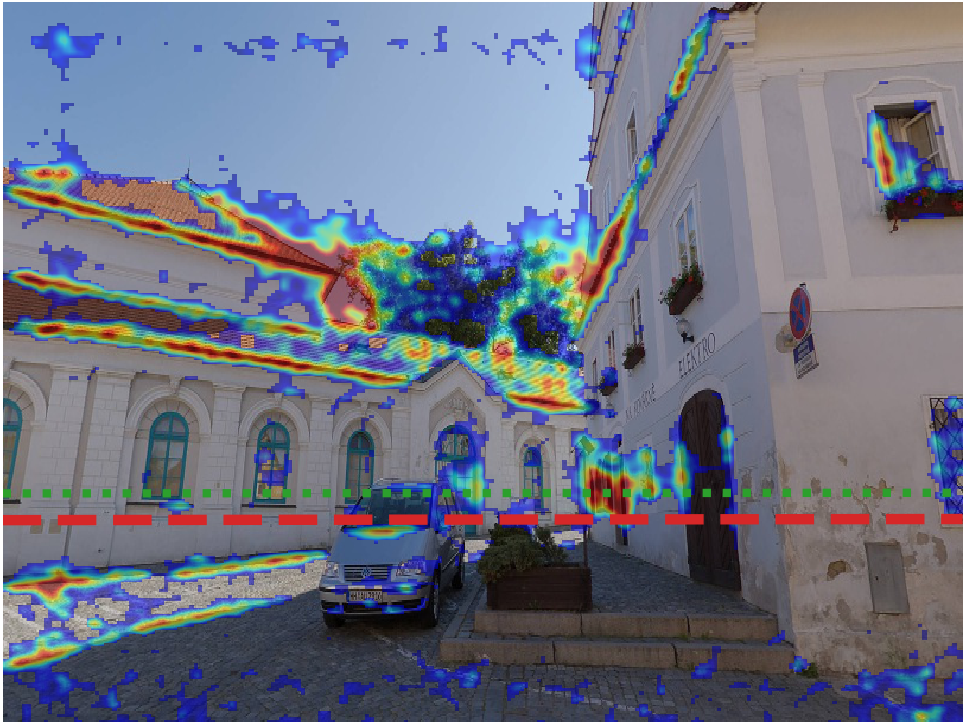
\includegraphics[width=\sgbpwidth\linewidth]{figures/nn_analysis/sgbp/pano_ayfpxlgzfcixnm_jpg-6.png} &
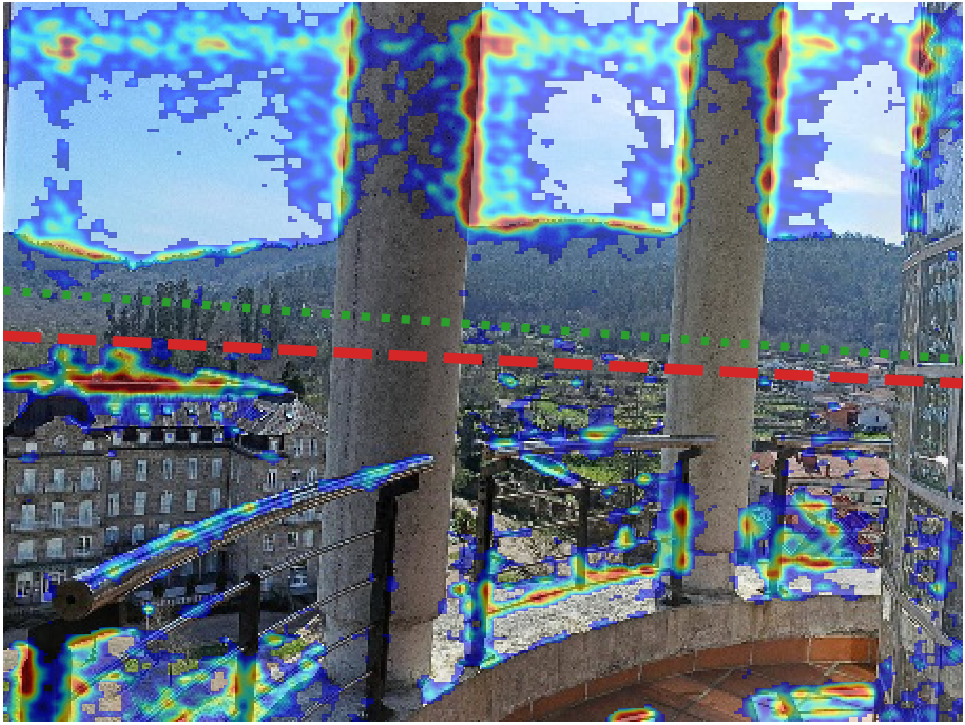
\includegraphics[width=\sgbpwidth\linewidth]{figures/nn_analysis/sgbp/pano_addontedcyafqk_jpg-6.png} &
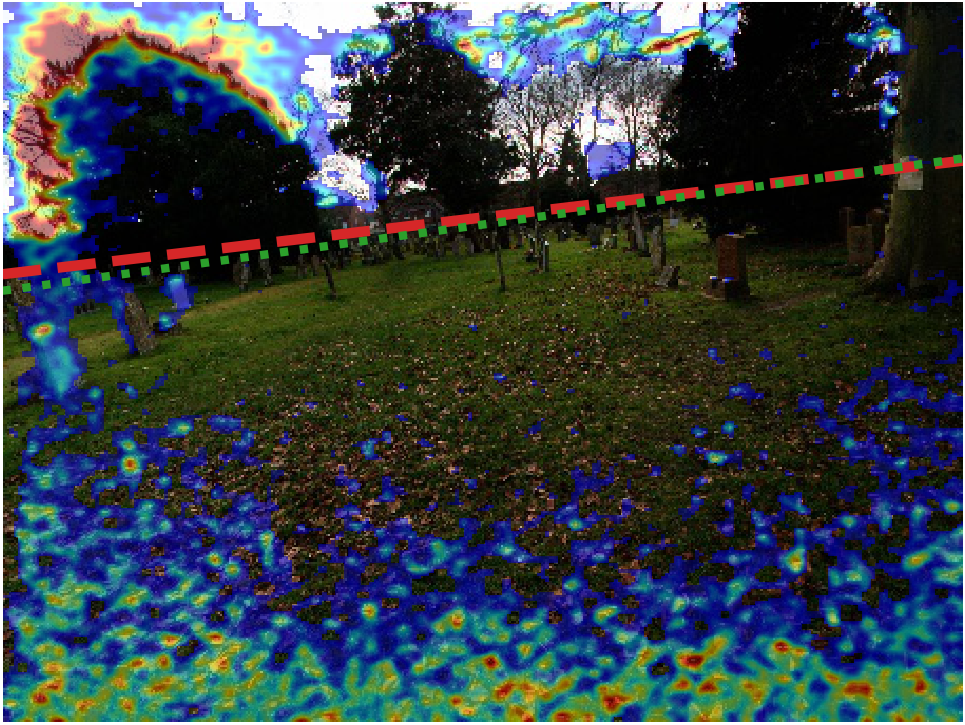
\includegraphics[width=\sgbpwidth\linewidth]{figures/nn_analysis/sgbp/pano_addhxkomphqrlr_jpg-4.png} \\
\multicolumn{5}{@{}c@{}}{
\includegraphics[trim={0 0.5cm 0.5cm 0},clip,width=0.3\linewidth]{figures/nn_analysis/sgbp/sgbp_colorbar.pdf}}
\end{tabular}
\egroup
\def\arraystretch{0.5} % this doesn't seem to do exactly what I want, but it does something
\caption[Analysis of the neural network focus]{\textbf{Analysis of the neural network focus.} The result of smoothed guided backpropagation is displayed as a jet overlay. When present, edges corresponding to important vanishing lines are highlighted while other edges are discarded. When no clear horizontal vanishing lines are detected, the neural network seems to look for the boundaries of either sky or land textures while dismissing the clouds or objects like trees, probably hinting bounds on horizon location in the image. \textbf{More examples available in annex~\ref{annex5}.}}
\label{fig:nn_analysis_smoothed-guided-back-propagation}
\end{figure*}


\paragraph{Feature analysis} We use guided backpropagation~\cite{Springenberg2015} to understand the image features our CNN-based method focuses on to perform its estimation. We use the smoothgrad~\cite{smilkov-arxiv-17} version of guided backpropagation (SGB) to obtain a more stable analysis. Qualitative results are shown in fig.~\ref{fig:nn_analysis_smoothed-guided-back-propagation}. Note how edges representing vanishing lines are highlighted by SGB in accordance to the features used by geometry-based approaches such as Upright. Sharp edges that are not useful for horizon estimation, such as clouds or organic objects,  are not taken into account. As such, we believe this focus map could help geometric-based approaches select the appropriate edges for geometric calibration estimation. Furthermore, when no clear vanishing line is detected in the image, the CNN model tends to focus on boundaries between sky and land, as the horizon typically lies on or below this boundary.
% YHG: ~\cite{Beardsley1992} <- they detect horizon lines by segmenting the sky, maybe not worth citing



%!TEX root = main.tex
\section{Evaluation}

\begin{figure}
\centering
\bgroup
\def\arraystretch{0}%  1 is the default, change whatever you need
\begin{tabular*}{\linewidth}{@{\hspace{1pt}}c@{\hspace{1pt}}c@{\hspace{1pt}}c@{\hspace{1pt}}c@{\hspace{1pt}}c@{\hspace{1pt}}c@{\hspace{1pt}}}

\vspace{2pt} 9:19 & 10:19 & 11:39 & 13:04 & 14:04 & 15:27 \\
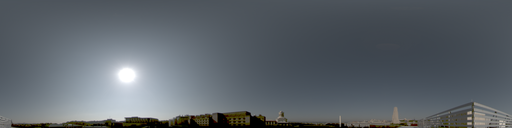
\includegraphics[width=0.16\linewidth]{figures/results/examples/20130621/091938.png} &
%\includegraphics[width=0.2\linewidth]{figures/results/examples/20130621/094937.png} &

\includegraphics[width=0.16\linewidth]{figures/results/examples/20130621/101936.png} &
%\includegraphics[width=0.2\linewidth]{figures/results/examples/20130621/104435.png} &
%\includegraphics[width=0.2\linewidth]{figures/results/examples/20130621/111434.png} &
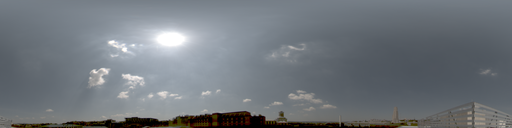
\includegraphics[width=0.16\linewidth]{figures/results/examples/20130621/113934.png} &
%\includegraphics[width=0.2\linewidth]{figures/results/examples/20130621/120933.png} &
%\includegraphics[width=0.2\linewidth]{figures/results/examples/20130621/123933.png} &

\includegraphics[width=0.16\linewidth]{figures/results/examples/20130621/130433.png} &
%\includegraphics[width=0.2\linewidth]{figures/results/examples/20130621/133432.png} &
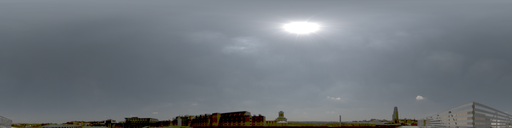
\includegraphics[width=0.16\linewidth]{figures/results/examples/20130621/140431.png} &
%\includegraphics[width=0.2\linewidth]{figures/results/examples/20130621/144650.png} &
%\includegraphics[width=0.2\linewidth]{figures/results/examples/20130621/145704.png} &
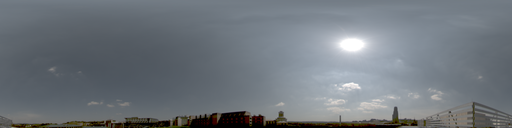
\includegraphics[width=0.16\linewidth]{figures/results/examples/20130621/152700.png} \\%\includegraphics[width=0.2\linewidth]{figures/results/examples/20130621/155157.png} &
%\includegraphics[width=0.2\linewidth]{figures/results/examples/20130621/161154.png} \\

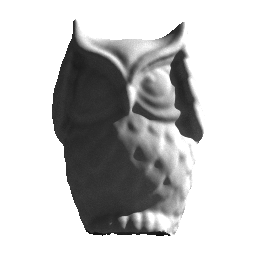
\includegraphics[width=0.16\linewidth]{figures/results/examples/20130621_inputs_owlie/img-01.png} &
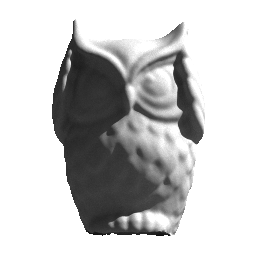
\includegraphics[width=0.16\linewidth]{figures/results/examples/20130621_inputs_owlie/img-03.png} &
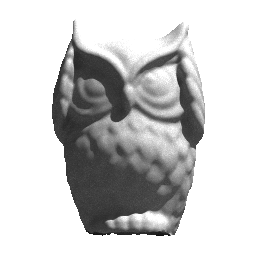
\includegraphics[width=0.16\linewidth]{figures/results/examples/20130621_inputs_owlie/img-06.png} &
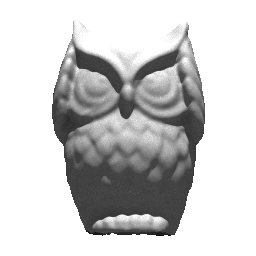
\includegraphics[width=0.16\linewidth]{figures/results/examples/20130621_inputs_owlie/img-09.png} &
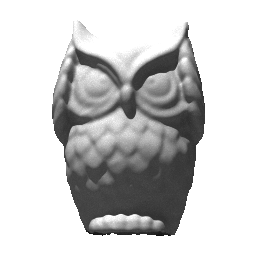
\includegraphics[width=0.16\linewidth]{figures/results/examples/20130621_inputs_owlie/img-11.png} &
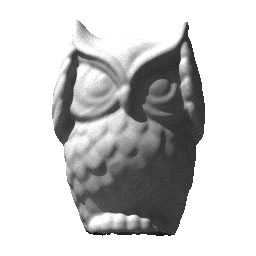
\includegraphics[width=0.16\linewidth]{figures/results/examples/20130621_inputs_owlie/img-14.png} \\
\end{tabular*}

\noindent\rule{0.95\linewidth}{0.4pt}
\newcommand{\reswidth}{0.141}
\begin{tabular*}{\linewidth}{@{}c@{}c@{}c@{}c@{}c@{}c@{}c@{}}

\includegraphics[width=\reswidth\linewidth]{figures/results/examples/gt_owlie_normals.png} &
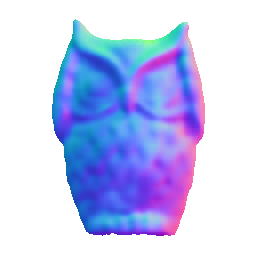
\includegraphics[width=\reswidth\linewidth]{figures/results/examples/ours_owlie_normals.png} &

\includegraphics[width=\reswidth\linewidth]{figures/results/examples/jung_owlie_normals.png} &
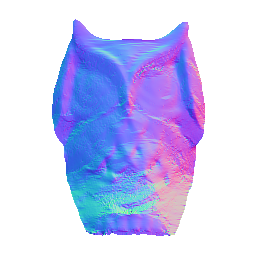
\includegraphics[width=\reswidth\linewidth]{figures/results/examples/yu_owlie_normals.png} &

\includegraphics[width=\reswidth\linewidth]{figures/results/examples/dpsn_owlie_normals.png} &
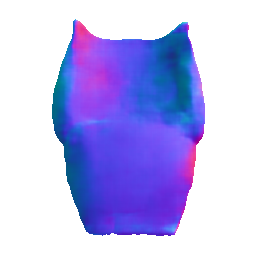
\includegraphics[width=\reswidth\linewidth]{figures/results/examples/marrnet_owlie_normals.png} &

\includegraphics[width=\reswidth\linewidth]{figures/results/examples/ef_owlie_normals.png} \\

\multicolumn{1}{r}{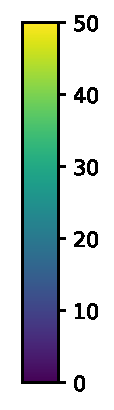
\includegraphics[height=\reswidth\linewidth]{figures/results/examples/colorbar_error_vertical.pdf}} &

\includegraphics[width=\reswidth\linewidth]{figures/results/examples/ours_owlie_errors.png} &
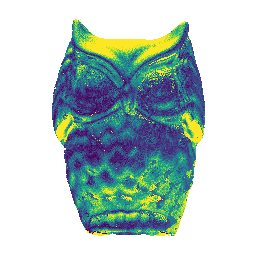
\includegraphics[width=\reswidth\linewidth]{figures/results/examples/jung_owlie_error.png} &
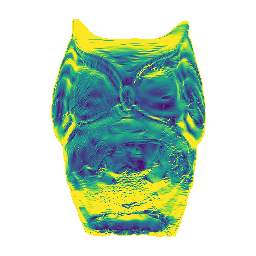
\includegraphics[width=\reswidth\linewidth]{figures/results/examples/yu_owlie_errors.png} &
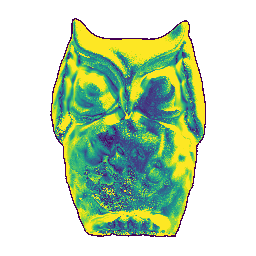
\includegraphics[width=\reswidth\linewidth]{figures/results/examples/dpsn_owlie_errors.png} &
\includegraphics[width=\reswidth\linewidth]{figures/results/examples/marrnet_owlie_errors.png} &
\includegraphics[width=\reswidth\linewidth]{figures/results/examples/ef_owlie_errors.png} \\

\includegraphics[width=\reswidth\linewidth]{figures/results/examples/gt_buddha_normals.png} &
\includegraphics[width=\reswidth\linewidth]{figures/results/examples/ours_buddha_normals.png} &
\includegraphics[width=\reswidth\linewidth]{figures/results/examples/jung_buddha_normals.png} &
\includegraphics[width=\reswidth\linewidth]{figures/results/examples/yu_buddha_normals.png} &
\includegraphics[width=\reswidth\linewidth]{figures/results/examples/dpsn_buddha_normals.png} &
\includegraphics[width=\reswidth\linewidth]{figures/results/examples/marrnet_buddha_normals.png} &
\includegraphics[width=\reswidth\linewidth]{figures/results/examples/ef_buddha_normals.png} \\

\multicolumn{1}{r}{\includegraphics[height=\reswidth\linewidth]{figures/results/examples/colorbar_error_vertical.pdf}} &
\includegraphics[width=\reswidth\linewidth]{figures/results/examples/ours_buddha_errors.png} &
\includegraphics[width=\reswidth\linewidth]{figures/results/examples/jung_buddha_error.png} &
\includegraphics[width=\reswidth\linewidth]{figures/results/examples/yu_buddha_errors.png} &
\includegraphics[width=\reswidth\linewidth]{figures/results/examples/dpsn_buddha_errors.png} &
\includegraphics[width=\reswidth\linewidth]{figures/results/examples/marrnet_buddha_errors.png} &
\includegraphics[width=\reswidth\linewidth]{figures/results/examples/ef_buddha_errors.png} \\
\begin{tabular}{@{}c@{}}ground\\truth\end{tabular} & ours & \cite{jung-cvpr-15} & \cite{yu-iccp-13} & \cite{santo-iccv-17} & \cite{wu-nips-17} & \cite{eigen-iccv-15} \\
\end{tabular*}
\egroup
\caption{(top) An example of the lighting environment maps and renders throughout a day. (bottom) Qualitative results (odd rows) and errors in degrees (even rows) of our technique and the state-of-the-art on single-day photometric stereo in the semi-calibrated~\cite{jung-cvpr-15} and calibrated~\cite{yu-iccp-13} cases, deep photometric stereo~\cite{santo-iccv-17} and single image normal estimation~\cite{wu-nips-17,eigen-iccv-15} (averaged over the day) on our real lighting dataset. \textbf{More results available in the supplementary material.}}
\label{fig:results-qualitative}
\end{figure}


In this section, we assess the performance of our method and compare it extensively to the state-of-the-art methods in single-day and regular photometric stereo, as well as some recent single image normal estimation techniques.

\subsection{Evaluation dataset}
\label{sec:evaluation_dataset}

To evaluate and compare the techniques, we rely on a dataset of synthetic objects, lit by real skies. To generate the images, we manually selected 3 sunny days over 2 geographical locations from the Laval HDR sky database~\cite{hdrdb}, which contains unsaturated HDR, omnidirectional photographs of the sky captured with the approach proposed in \cite{stumpfel-afrigraph-04}. We build a virtual 3D scene containing the HDR sky environment map as the sole light source, a 3D object viewed by an orthographic camera, and a 0.3 albedo ground plane placed under the object, outside the field of view of the camera. We used the 3D models from the validation set which the neural network never saw during training. This results in a dataset of 960 renders yielding 60 normal maps to evaluate. Example images obtained with this technique are shown in fig.~\ref{fig:results-qualitative}. 

% High dynamic range (HDR) captures of the sky hemisphere that span the full 22 stops required to properly capture outdoor lighting were taken using the approach proposed in~\cite{stumpfel-afrigraph-04}. We captured three different sunny days over two different geographical locations. 

%Days used: 2013-06-21 (Pittsburgh), 2015-05-14 and 2016-06-17 (Québec City). The sun has a maximum elevation of $73.00\degr$, $61.86\degr$ and $66.59\degr$, respectively.


\subsection{Results and comparisons}

We compare our method to several state-of-the-art techniques relying on photometric stereo and/or deep learning to estimate surface normals from images. For PS techniques, we compare to the calibrated technique of Yu et al.~\cite{yu-iccp-13}, which requires knowledge of the full environment map used to light the object. In our work, we use the variant proposed by Hold-Geoffroy et al.~\cite{holdgeoffroy-3dv-15} and without the low-rank matrix completion preprocessing, which was shown to yield slightly improved results over the original formulation. We also compare to the semi-calibrated method of Jung et al.~\cite{jung-cvpr-15}, which requires only knowledge of the capture geolocation. For deep learning techniques, we compare to the recent Deep Photometric Stereo Network (DPSN)~\cite{santo-iccv-17}, which operates on one pixel at a time. Since it assumes known point light source lighting, we re-trained this model using the sun position from a geographical location and date representative of our training dataset. In addition, we also compare to single image networks: Eigen and Fergus~\cite{eigen-iccv-15} and MarrNet~\cite{wu-nips-17}. Since they rely on a single image, we take the mean of their results averaged over all 8 inputs. 

The comparative results, shown qualitatively in fig.~\ref{fig:results-qualitative} and quantitatively in fig.~\ref{fig:results-quantitative}, clearly demonstrate that our approach significantly outperforms all other techniques. We observe that both single image techniques do not work well and result in very high median errors of around $40\degr$ and $70\degr$ for~\cite{wu-nips-17} and \cite{eigen-iccv-15}, respectively. For \cite{eigen-iccv-15}, this is probably due to the fact that they cannot handle the harsh shadows created by outdoor lighting during sunny days, since they train with indoor lighting only. In addition, MarrNet~\cite{wu-nips-17} outputs a voxel occupation grid and only produces normals as a byproduct (in its latent stage). As such, this method may not be fully optimized for normal estimation.

The PS techniques yield much better results but still yield quite significant error since sunny days do not contain sufficient constraints to accurately recover surface normals. The calibrated method of Yu et al.~\cite{yu-iccp-13} is comparable to the results obtained by DPSN, with a median normal angular estimation error of $33\degr$. Interestingly, the semi-calibrated method of Jung et al.~\cite{jung-cvpr-15} actually yields better results with a median error of $22\degr$, despite needing less information than the calibrated methods. This could be due to its reliance on a parametric clear sky model to estimate lighting, which closely matches the actual ground truth lighting, and to its reliance on an intensity profile matching algorithm.


\begin{figure}[t]
\centering
\includegraphics[width=0.75\linewidth]{figures/results/real_lighting_performance.pdf}
\caption{Median reconstruction error on our real lighting dataset displayed vertically as “box-percentile plots”~\cite{esty-jss-03}; the center horizontal bars indicate the median, while the bottom (top) bars are the 25th (75th) percentiles. Our proposed method (green) provides state-of-the-art performance compared to non-learned methods for single-day PS (blue~\cite{jung-cvpr-15}, orange~\cite{yu-iccp-13}), deep learning methods on calibrated photometric stereo (red~\cite{santo-iccv-17}) and single image normals reconstruction (purple~\cite{wu-nips-17}, brown~\cite{eigen-iccv-15}).}
\label{fig:results-quantitative}
\end{figure}

It is interesting to note that most PS techniques capture with some degree of success the left/right component of the surface normals (roughly speaking, the red and blue tints in the normal maps). This axis happens to be the same as the sun trajectory through the day when the camera is facing north or south. This results in strong photometric constraints on this axis. On the other hand, the recovery of the up/down axis is much less successful on most techniques as outdoor photometric cues lack information in this direction through a single sunny day.

In contrast, our method yields a normal map that is, although a bit smoother, qualitatively very similar to the ground truth. Quantitatively, our approach achieves a median error of $14\degr$ over the evaluation set, with the majority of errors being completely below that of the next-best performing method, Jung et al.~\cite{jung-cvpr-15} (see fig.~\ref{fig:results-quantitative}). Even if it is trained on purely synthetic data, our network is able to generalize well to images rendered with real lighting. The difference in performance with respect to DPSN shows the usefulness of dealing with image patches, which allows the network to learn appropriate patch-based shape priors which can be exploited when the photometric cue alone is not sufficient. 

% deep learning based photometric stereo~\cite{santo-iccv-17} as well as two recent single image normals estimation techniques: Eigen and Fergus~\cite{eigen-iccv-15} and MarrNet~\cite{wu-nips-17}. Qualitative results as well as quantitative results on median estimation error are shown in fig.~\ref{fig:experimental_results}-~\ref{fig:performance_real_lighting}, respectively. We observe that our proposed method outperforms previous work the vast majority of the time.


% Deep Photometric Stereo Network (DPSN)~\cite{santo-iccv-17} needs fully calibrated lighting positions. To evaluate on the one-day case, we trained this model using the sun position from a random geographical location and date. The model overfitted to this specific lighting pattern and did not adapt to different geographical locations and dates.

% In the case of~\cite{jung-cvpr-15}, the performance is reported on a subset of 2 objects over 2 days, and the MRF refinement post-processing was not performed. % Calibrated one-day photometric stereo~\cite{yu-iccp-13} was performed without the low-rank matrix completion preprocessing.

% ~\cite{yu-iccp-13,santo-iccv-17,jung-cvpr-15} all infer normals by looking at the photometric cues from a single pixel at a time. We argue that spatiality is important for one-day photometric stereo as it improves the signal-to-noise ratio in the axis perpendicular to the sun path through the day.



%\begin{figure}
%\centering
%\includegraphics[width=0.49\linewidth]{figures/analysis/perfs_per_direction_normal.pdf}
%\includegraphics[width=0.49\linewidth]{figures/analysis/perfs_per_direction_16divs.pdf}
%\hspace*{0.7cm}\begin{tabular*}{0.55\linewidth}{c@{\extracolsep{\fill}}c}
%(a) & (b)
%\end{tabular*} \\
%\caption{Reconstruction performance on our synthetic test dataset in function of the ground truth surface normal direction for our model with regular image input (a) and denominator images input (b).
%\todo{Should we keep this figure?}}
%\label{fig:surface_normal_direction}
%\end{figure}


%!TEX root = main.tex
\section{Analysis}
\label{sec:analysis}

We now analyze further our network, and in particular explore the robustness of our network to departures from the assumptions that were made in sec.~\ref{sec:proposed_method}. 

\subsection{Camera calibration error}

To constrain the set of possible lighting directions (sec.~\ref{sec:analemma}), we made the assumption that the camera is pointing north. We analyzed the impact on reconstruction performance when this hypothesis is infringed by rotating the real environment maps used to render the evaluation dataset (sec.~\ref{sec:evaluation_dataset}), and show the results of this experiment in fig.~\ref{fig:calibration_error_performance}. The slight improvement around $5\degr$ west calibration error is due to the timestamps of our real lighting dataset that are not perfectly aligned with the neural network expected timestamps. We observe that the median reconstruction error increases of approximately $5\degr$ per $10\degr$ error on camera calibration, showing that the network has some built-in robustness to these errors. 


\begin{figure}[!t]
\centering
\includegraphics[width=0.7\linewidth]{figures/analysis/performance_calibration_error.pdf}
\caption{Median normal estimation error as box-percentile plots (see fig.~\ref{fig:results-quantitative}) in function of the camera deviation from north in degrees on our real lighting dataset. Positive means camera going toward west, negative means camera going toward east. }
\label{fig:calibration_error_performance}
\end{figure}


\subsection{Number of images}
\label{sec:ablation_study}

We now study the normal estimation performance in function of the number of inputs $T$ to the CNN (see sec.~\ref{sec:architecture}). Results ranging from a single input image ($T=1$, effectively performing shape-from-shading) to $T=16$ input images all uniformly taken from 9:00 to 16:00 are shown in fig.~\ref{fig:number_of_inputs}. We observe an rapid improvement in performance from one to three images, which is coherent with Photometric Stereo theory~\cite{woodham-opteng-80}. Performance continues to increase until $T=8$, probably because added constraints improves robustness to noise and non-diffuse materials. Interestingly, the normal estimation error starts to increase slightly with $T > 8$. This could be due to an increase in the number of parameters to train in our model (the output tensor after concatenation is of dimension $14 \times 14 \times 32T$, thereby increasing the number of parameters in the second convolutional layer), making the model harder to train.

% It is interesting to note the performance of the single image case, where the model obtains better than 24 degree median reconstruction error for half the renders, which is still quite competitive.


\begin{figure}[!t]
\centering
\includegraphics[width=0.75\linewidth]{figures/analysis/input_ablation.pdf}
\caption{Median normal estimation error as box-percentile plots~\cite{esty-jss-03} (see fig.~\ref{fig:results-quantitative}) on our evaluation dataset as a function of $T$, the number of input images.}
\label{fig:number_of_inputs}
\end{figure}


\subsection{Feature analysis}

We use SmoothGrad~\cite{smilkov-arxiv-17} to visualize the regions of the image that have a larger impact on normal estimation. Since the network operates on patches and not entire images, we use the same linear blending strategy as in sec.~\ref{sec:training_dataset}, and report qualitative results in fig.~\ref{fig:smoothgrad}. We observe how the neural network tends to ignore darker regions and focuses on brighter alternatives in other images when available. This result suggests that the network learns to avoid shadowed areas, where, indeed, the photometric cue is not reliable due to low signal-to-noise ratio and to occlusion of the main light source.


\begin{figure}[!t]
\centering
\includegraphics[width=0.49\linewidth]{figures/analysis/smoothgrad_inputs.png}
\includegraphics[width=0.49\linewidth]{figures/analysis/smoothgrad.png} \\
\vspace{-1em}
\hspace*{-0.1cm}\begin{tabular*}{\linewidth}{c@{\extracolsep{\fill}}c}
 & \includegraphics[width=0.46\linewidth]{figures/analysis/colorbar_smoothgrad_horizontal.pdf}
\end{tabular*} \\
\vspace{-0.7em}
\hspace*{0.4cm}\begin{tabular*}{0.53\linewidth}{c@{\extracolsep{\fill}}c}
(a) & (b)
\end{tabular*} \\
\caption{Back-propagating the gradient through our network using SmoothGrad~\cite{smilkov-arxiv-17} on the input images shown in (a) generates a map of the pixels that affects the most the normal estimation (b). Notice how the regions in shadow have generally less influence (blue) than regions in direct sunlight (yellow).}
\label{fig:smoothgrad}
\end{figure}


%!TEX root = main.tex
\chapter*{Conclusion}         % ne pas numéroter
\phantomsection\addcontentsline{toc}{chapter}{Conclusion} % dans TdM


Throughout this thesis, we show that gathering and analyzing large datasets can bring new insights that can both improve classical methods and build advanced machine learning algorithms. Three main axes of research were presented. First, we proposed a framework to analyze the performance of outdoor Photometric Stereo, which can explain the reasons leading to accurate tridimensional surface reconstruction through photometric signal under daylight. Using this framework, we demonstrated that partially cloudy days are more suited to perform outdoor PS from photometric signal alone. We also showed that clear days typically do not yield enough photometric information to perform a robust surface reconstruction. We then presented a learning-based method that augments photometric cues with priors to solve the instability of the PS problem during sunny days. Secondly, we proposed a single image learning-based algorithm for outdoor lighting estimation that is robust to various scene content and exhibits state-of-the-art performance. We achieved this by fitting the physics-based Ho\v{s}ek-Wilkie sky model to a large dataset of 360$\degr$ panoramas and used it to train our machine learning model. Lastly, we used a similar approach to create a camera calibration method, which estimates automatically the field of view and the position of the horizon within the image. These last two methods can be used to streamline compositing operations by enabling automatic photorealistic virtual object insertion and relighting, along with applications like image retrieval. All proposed methods work on generic scenes and rely heavily on the priors modeled directly from the training data. 

For every project presented, we strove to understand the underlying patterns in the data. We proposed a framework for photometric stereo sensitivity analysis, which can predict reconstruction performance from the sky appearance. We also experimented with our surface reconstruction approach under various configurations to better understand the impact of camera calibration error and the number of input images on the reconstruction performance. Furthermore, the proposed camera calibration estimation method was analyzed through guided backpropagation, which allowed us to better understand the visual cues picked up by the learned model. Even though deep learning models are generally considered \emph{black boxes} by the community, we hope our efforts in explaining the behavior of those machine learning methods have inspired others to continue in this direction.

All approaches described in this thesis have direct applications in entertainment and advertisement, notably by enabling photorealistic virtual object insertion and relighting automatically. The lighting estimation and camera calibration techniques presented in this thesis (see chapters~\ref{ch3} and~\ref{ch4}) received worldwide recognition and were implemented into Dimension, the new 3D editing software from Adobe Systems. Thanks to these new technologies, multimedia artists are reporting their increased productivity and reduced time needed to create or modify works, as shown in the following testimony from a user: ``One of the greatest features is Dimension's ability to derive lighting from an image [and] use that to light an object. Results are amazing.'' In addition to its influence on digital media artists, the techniques proposed in this thesis also had an impact on the scientific community. We notably won the \emph{Best Paper (Runner Up)} award in 2015 for the work presented in chapter~\ref{ch1}, which analyzed and improved outdoor surface reconstruction techniques. This technique can also have a large-scale impact, as it can be used to perform 3D scans of large statues and buildings, where hand-held scanning would take a prohibitive amount of time. The video game and movie industries use similar techniques to digitize actors~\cite{debevec2000acquiring} to produce photorealistic alter-egos. Using our proposed approach, the same could be done for large-scale elements like buildings and would allow studios to easily obtain high fidelity models for their creations. Aside from the entertainment industry, this technique can allow the preservation of cultural heritage of statues and buildings through digital copies that will stand the test of time. Additionally, the light and camera parameters estimation techniques we developed can also provide additional information to sensors, improving the quality of information provided by decision support systems. Similarly, our approaches could complement robot navigation and localization systems by providing another source of attitude estimation based on visual cues. Image forensics can also benefit from the ideas proposed in this thesis: detecting shadow orientations (by estimating sun position) and detecting conflicting horizons can help discover image modifications~\cite{Farid2010}. As can be seen, modeled priors can be used to perform hard computer vision tasks and have a myriad of applications. It is our hope that this thesis has brought some insights and tools to enable the next generation of deep learned priors to computer vision tasks. 



\bibliographystyle{splncs}
\bibliography{bibliography}
\end{document}
